\chapter{Método proposto} 
\label{sec:metodo}

Neste capítulo estudaremos uma abordagem em dois níveis para a complementação automática de consulta tolerante a erros que usa o algoritmo \textit{ICPAN} no primeiro nível, e usa tanto pesquisa sequencial quanto binária no segundo nível. O primeiro nível serve como um filtro que seleciona candidatos à resposta para serem processados no segundo nível, responsável por determinar quais candidatos são qualificados como resposta final.

O intuito dessa abordagem é reduzir o uso de memória e ao mesmo tempo manter o desempenho quanto ao tempo de processamento da consulta. Os sistemas de busca podem se beneficiar dessa redução pois ela possibilita diminuir os custos com memória mantendo o mesmo conjunto de dados, ou então pode permitir o aumento do conjunto de dados sem que haja um grande impacto na quantidade de memória usada pelo método.

Seja $\mathcal{D}$ a base de dados considerada nos parágrafos a seguir, composta pelos seguintes itens: \textit{\{insects, integer, integral, integrity, intellect, intelligent, invest, invested, investigate, telepathic, telepathy, telephone, telephoto, teleport, teleprompter\}}. Atribuímos um valor de $id$ a cada item, partindo do número $0$, como é possível observar na tabela de itens da Figura~\ref{fig:index_structure}. A etapa de indexação considera que todos os itens estão ordenados em ordem lexicográfica crescente, e para que os exemplos fiquem mais simples cada item contém apenas uma palavra.
 
\section{Indexação} 
\label{sec:indexing}
Seja $w$ a cadeia de caracteres de um item, $|w|$ o tamanho da cadeia, e $w[i]$ uma indicação do $i$-ésimo caractere de $w$, com $i=1$ referindo-se ao primeiro caractere. A expressão $w[i..j]$ representa uma subcadeia de caracteres de $w$ começando na $i$-ésima posição e terminando na $j$-ésima. Consideramos também que se $j > |w|$, então $w[i..j] = w[i..|w|]$, e também que $w[i..]$ representa a subcadeia que começa no $i$-ésimo caractere, e termina no último caractere de $w$. Sendo assim, para $w = ``sapato"$, temos que $w[3..27] =  ``pato"$ e $w[4..] = ``ato''$, por exemplo.  

 
 \begin{figure} [ht]
    \centering
    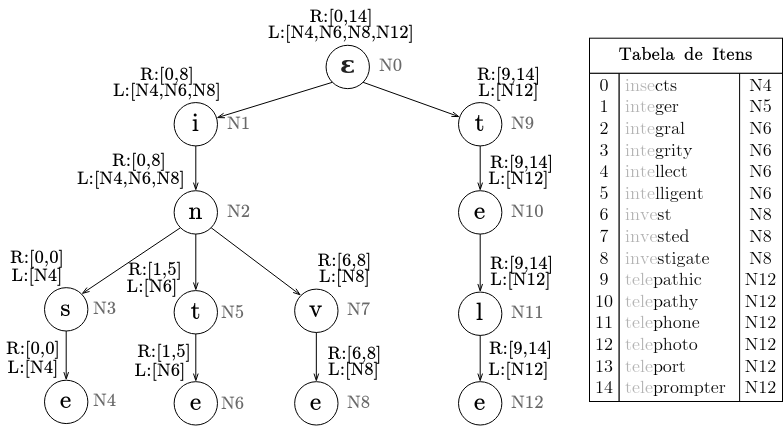
\includegraphics[width=0.94\textwidth]{figures/index-structure.png}
    \caption{Árvore \textit{Trie} com os prefixos de tamanho $\lambda = 4$ indexados, na qual cada nó possui intervalos $R$ de \textit{ids} e listas $L$ de nós folha dentre os seus descendentes.}
    \label{fig:index_structure}
\end{figure}

 
Como parte da implementação da estrutura proposta, indexamos as descrições textuais dos itens em uma árvore \textit{Trie} $\mathcal{T}$ mantida em memória. Seja também $\lambda$ a altura máxima permitida para $\mathcal{T}$, considerando que o nível do nó $\epsilon$ (nó $N0$ na Figura~\ref{fig:index_structure}) é igual a $0$. Dessa forma, o nó $N7$ tem altura igual a $3$, por exemplo. Para cada cadeia $w$ de um item inserimos em $\mathcal{T}$ apenas o prefixo $Prefixo_{\lambda}(w)$, onde $Prefixo_{\lambda}(s) = s[1..\lambda]$ é uma função que retorna os $\lambda$ primeiros caracteres da cadeia $s$ passada como parâmetro.

Cada nó $n$ em $\mathcal{T}$ contém um caractere $n.caractere$, um número de identificação $n.id$, e a sua altura $n.altura$ correspondente na árvore (sendo a altura do nó $\epsilon$ igual a 0). Também possui um intervalo $n.R = [menor, maior]$ no qual $menor$ e $maior$ representam respectivamente o menor e o maior $id$ dos itens em $\mathcal{T}$ que compartilham o mesmo prefixo $p_{n}$ obtido ao caminhar partindo do nó $\epsilon$ até $n$. Esse intervalo é análogo à lista invertida mencionada no fim da seção~\ref{sec:icpan_algorithm_description}. Para uma subárvore com raiz no nó $n$, todos os itens nessa subárvore irão compartilhar o mesmo prefixo $p_{n}$. Objetivando a simplicidade, iremos nos referir a $n$ pelo seu prefixo $p_{n}$ correspondente de forma intercambiável, assim como foi feito na seção~\ref{sec:trie}. 

Por fim, cada nó $n$ possui uma lista $n.L$ que contém todos os nós folha de sua subárvore. Quando o próprio $n$ é uma folha, não possui subárvore, então a lista conterá apenas o próprio $n$, ou seja, $n.L = [n.id]$.

A Figura~\ref{fig:index_structure} mostra uma \textit{Trie} $\mathcal{T}$ após a indexação dos $\lambda = 4$ primeiros caracteres de cada item em $\mathcal{D}$. Também mantém-se uma estrutura de dicionário $\mc{H}$, representada pela ``Tabela de Itens'', que mapeia o valor do \textit{id} de um item ao texto do restante da sua descrição, ou seja, $w[5..]$ (texto após o 4º caractere).

Essa estrutura é utilizada para reconstruir a descrição completa de um item a partir de qualquer nó de prefixo \textit{p}. Apesar da Figura~\ref{fig:index_structure} mostrar o texto completo de cada item na ``Tabela de Itens'', os $4$ primeiros caracteres em cinza claro são na verdade obtidos ao caminhar por $\mathcal{T}$. Para possibilitar essa reconstrução, também guardamos em $\mc{H}$ o $id$ do nó correspondente ao prefixo $Prefixo_{\lambda}(w)$ do item. Supondo por exemplo a reconstrução de ``\textit{investigate}'', com $id=7$ em $\mc{H}$, basta processar o prefixo $p$ do nó $N8$, que é \textit{p = ``inve''}, como mostra a Figura~\ref{fig:index_structure}, e então concatenar $p$ com ``\textit{stigate}'', que é o conteúdo presente em $\mc{H}$ para a chave $id=7$.

\begin{algorithm}[ht]
\caption{Construção de um índice \textit{Trie} $\mc{T}$ a partir de sugestões de consultas de uma base $\mc{D}$}\label{alg:dataset_indexing}
\begin{algorithmic}[1]
\Function{ConstruirIndiceTrie}{$\mc{D}, \mc{H}, \mc{T}$}
    \For{$Q \in \mc{D}$}
        \State $item.noPrefixo \leftarrow inserirPrefixo(\mc{T}, Prefixo_{\lambda}(Q.texto), Q.id)$
         \If{$|Q.texto| < \lambda$}
            \State $item.restante \leftarrow \epsilon$
         \Else{}
            \State $item.restante \leftarrow Q.texto[(\lambda + 1)..]$
         \EndIf
         
         \State $\mc{H}[Q.id] \leftarrow item$
    \EndFor
    \State $construirListasDeFolhas(\mc{T})$
\EndFunction
\end{algorithmic}
\end{algorithm}

O Algoritmo~\ref{alg:dataset_indexing} descreve a construção de um índice \textit{Trie} a partir de uma base de sugestões de consulta. Esse algoritmo tem como parâmetro: $\mc{D}, \mc{H}, \mc{T}$, os quais representam, respectivamente, a base de dados com as sugestões de consulta que serão indexadas, a estrutura de dicionário mencionada anteriormente, e a árvore \textit{Trie} ainda vazia. Esse algoritmo assume que os itens da base $\mc{D}$ estão em ordem lexicográfica crescente. O laço de repetição da linha 2 define o procedimento feito para cada sugestão de consulta $Q$ da base $\mc{D}$. Na linha 3, chama-se a função $inserirPrefixo$ (que será detalhada a seguir), a qual insere o prefixo $Prefixo_{\lambda}(Q.texto)$ (primeiros $\lambda$ caracteres do texto da sugestão de consulta) na \textit{Trie}, e retorna o nó da \textit{Trie} referente ao prefixo inserido. Então, esse nó é atribuído ao atributo $noPrefixo$ do $item$. Na linha 4, há uma condição para verificar se o tamanho do texto de $Q$ é menor que $\lambda$. Se for, então o atributo $restante$ do $item$ recebe o valor de texto vazio $\epsilon$, na linha 5. Senão, recebe o valor do restante do texto de $Q$ após o $\lambda$-ésimo caractere, na linha 7. Com o item já montado, associa-se a chave $Q.id$ com o $item$ no dicionário $\mc{H}$ na linha 8, e o laço de repetição segue para a próxima sugestão de consulta de $\mc{D}$, se houver. Após o termino do laço, chama-se a função $construirListasDeFolhas$ na linha 9. Essa função itera sobre cada nó $n$ da \textit{Trie}  $\mc{T}$, preenchendo as listas $n.L$ de cada nó, as quais contêm todos os nós folha com raiz em $n$.


\begin{algorithm}[H]
\caption{Inserção de um prefixo de sugestão de consulta em $\mc{T}$}\label{alg:append_prefix_trie}
\begin{algorithmic}[1]
\Function{inserirPrefixo}{$\mc{T}, prefixo, id$}
    \State $raiz \leftarrow obterRaiz(\mc{T})$d
    \State $n \leftarrow raiz$
    \State $raiz.R.maior = id$
    \For{$caractere \in prefixo$}
        \State $n \leftarrow n.inserirFilho(caractere, id)$
    \EndFor
    \State $n.marcadoFolha \leftarrow Verdadeiro$
    \State $n.L.inserir(id)$
    \State \textbf{return} $n$
\EndFunction
\end{algorithmic}
\end{algorithm}

O Algoritmo~\ref{alg:append_prefix_trie} descreve a inserção de um prefixo de sugestão de consulta (o qual pode na verdade ser a consulta inteira). Esse algoritmo tem como parâmetro: $\mc{T}, prefixo, id$, os quais representam a árvore \textit{Trie}, o prefixo de sugestão de consulta, e a identificação numérica da consulta, respectivamente. Na linha 4, atualiza-se o valor $maior$ do intervalo $raiz.R = [menor, maior]$ para ser igual ao $id$ da sugestão de consulta que está sendo inserida. Então, cada caractere do $prefixo$ (linha 5) é inserido na \textit{Trie} um a um na (linha 6). A cada inserção, o nó $n$ é atualizado com último nó que foi inserido ou apenas percorrido (caso todo o caminho já exista na árvore). Após essas inserções, na linha 8 o nó $n$ é marcado como folha. Por fim, o $id$ da sugestão de consulta é inserido na lista $L$ do nó $n$ na linha 9 e a função retorna $n$ na linha 10. 

\section{Algoritmo geral da abordagem em dois níveis}
\label{sec:general_two_level_algorithm}
% Esta premissa descrita a seguir não é 100% correta. Percebi no dia 26-05-2021 enquanto escrevia aqui que, com a implementação do conjunto de folhas virtuais, é possível computar nós ativos para os lambda+tau primeiros caracteres de p, ou para p inteiro caso |p| <= lambda + tau. Creio que vale a pena explorar essa premissa melhorada para a publicação do artigo.
Como descrito na seção~\ref{sec:indexing}, somente os $\lambda$ primeiros caracteres de cada sugestão de consulta da base são indexados na \textit{Trie}. Então, devido a esse fato, temos a premissa de que somente os $\lambda$ primeiros caracteres de um prefixo de consulta $p$ devem ser considerados na computação do conjunto de nós ativos. Com tal conjunto computado, cada nó é visitado, e recupera-se sua lista de nós folha. Para cada uma das listas invertidas desses nós folha, é possível realizar a busca sequencial apresentada na seção~\ref{sec:sequential_search}. 

\begin{algorithm}[H]
\caption{Algoritmo geral do processamento em dois níveis}\label{alg:general_two_level}
\begin{algorithmic}[1]
\Function{processarConsultaDoisNiveis}{$\mc{T}, p, \tau$}
    \If{$|p| + \tau \leq \lambda$} \textbf{return} $MetodoCATE(\mc{T},p,\tau)$
    \EndIf
    \State $sugestoes \leftarrow \emptyset$
    \State $nosAtivos \leftarrow computarNosAtivos(\mc{T}, Prefixo_{\lambda}(p), \tau)$ \Comment{Primeiro Nível}
    \For{$n \in nosAtivos$} \Comment{Segundo Nível (até a linha 6)}
        \For{$n_{folha} \in n.L$}
            \State $sugestoes \leftarrow sugestoes \cup buscaSequencial(p, n_{folha}.R, \tau)$
        \EndFor
    \EndFor
    \State \textbf{return} $sugestoes$
\EndFunction
\end{algorithmic}
\end{algorithm}

O Algoritmo~\ref{alg:general_two_level} é uma representação geral da abordagem em dois níveis para o problema de CATE. Ele tem como parâmetros $\mc{T}, p$ e $\tau$, os quais representam um índice \textit{Trie}, um prefixo de consulta, e o limiar de erros de digitação, respectivamente. O algoritmo tem início na linha 2 com uma verificação da condição $|p| + \tau \leq \lambda$, ou seja, se o tamanho do prefixo de consulta mais o número de erros de digitação tolerados é menor do que a altura máxima do índice \textit{Trie}.
Quando essa condição é verdade é possível utilizar somente o algoritmo de CATE (representado pela função \textit{MetodoCATE}) para computar todos os resultados para $p$, sem a necessidade de ativar o segundo nível. O prefixo de consulta pode sofrer no máximo $\tau$ inserções como erros de digitação, e se esse tamanho máximo ($|p| + \tau$) estiver dentro do limite $\lambda$, os nós indexados na \textit{Trie} são o suficiente para responder à consulta. Essa lógica estará presente também nos Algoritmos \ref{alg:ip2l} e \ref{alg:ip2lb}, com o método ICPAN sendo executado.

Caso a condição seja falsa, o algoritmo segue com o processamento em dois níveis. O conjunto de resposta $sugestoes$ é iniciado como vazio na linha 3, o qual conterá no fim da execução as sugestões de consultas com prefixos similares a $p$ considerando uma diferença de distância de edição de no máximo $\tau$. Na linha 4, é executada a função $computarNosAtivos$, que computa o conjunto de nós ativos da \textit{Trie} $\mc{T}$ para o prefixo $Prefixo_{\lambda}(p) = p[1..\lambda]$ considerando o limiar $\tau$. O algoritmo utilizado para tal computação pode ser, em tese, qualquer um baseado em processamento de nós ativos de árvores \textit{Trie}, como por exemplo o ICAN, ICPAN, ou BEVA. O conjunto final de nós ativos é armazenado na variável $nosAtivos$. Essa etapa caracteriza o primeiro nível. 

A linha 5 caracteriza o início do processamento do segundo nível. Nela há um laço de repetição que itera sobre cada nó ativo do conjunto $nosAtivos$, e na linha 6, há outro laço que itera sobre cada nó folha com raiz em $n$. Então, na linha 7, a função $buscaSequencial$ determina quais dentre as sugestões de consultas referenciadas pelo intervalo $R$ de $n_{folha}$ são respostas válidas, e então essas sugestões são unidas com o conjunto final de respostas. O algoritmo dessa função é o descrito na seção~\ref{sec:sequential_search}. Por fim, na linha 8 o conjunto de respostas é retornado.



\section{Primeiro nível}
\label{sec:first-level}

O algoritmo de busca utilizado no primeiro nível será o ICPAN, proposto por Li et al \citep{li2011efficient}. Como descrito no capítulo~\ref{sec:ref_teorico} o ICPAN utiliza um algoritmo incremental que calcula os prefixos semelhantes a um prefixo consultado, tolerando uma quantidade de erros de digitação previamente definida como o limite de distancia de edição $\tau$. Uma característica desse algoritmo é a ``ativação'' de nós da \textit{Trie} que correspondem a um prefixo que pode ser obtido considerando erros no prefixo consultado.

Ao considerar a utilização do ICPAN no primeiro nível, é preciso atentar para dois pontos: (1) uma vez que o primeiro nível serve apenas como filtro para o processamento do segundo nível, o algoritmo computará nós (pivô) ativos referentes a prefixos semelhantes a uma parte $p[1..\lambda]$ de um prefixo de consulta $p$, e não semelhantes a $p$ por completo. Esse conjunto será referido como $\Psi_{p[1..\lambda]}$ daqui em diante; (2) uma premissa da concepção original desse algoritmo é que todo o texto da sugestão de consulta estará indexado na \textit{Trie}, o que não acontece na abordagem em dois níveis.

Dessa maneira, o propósito original de utilização dos nós ativos foi modificado. Alguns nós importantes para o processamento no segundo nível acabam sendo desativados durante o processamento incremental do ICPAN, e deixam de estar presentes em $\Psi_{p[1..\lambda]}$. A partir dessa situação observamos em nossa pesquisa que o conteúdo do conjunto $\Psi{p[1..\lambda]}$ resultante da computação original do ICPAN \textit{não é suficiente para resolver completamente o problema de CATE na abordagem em dois níveis}. 

\subsection{Conjunto de nós folha virtuais ativos}
\label{sec:virtual_leaves_node-set}

Devido ao problema de nós desativados mencionado acima, faz-se necessário um mecanismo que preserve esses nós ativos importantes para que eles também estejam no conjunto final de nós ativos de $p[1..\lambda]$. O mecanismo proposto neste trabalho para resolver esse problema consiste em computar, simultaneamente ao conjunto de nós ativos $\Psi$ do ICPAN, um conjunto $\psi$ de ``nós folha virtuais ativos'' auxiliar que manterá esses nós importantes que acabariam sendo desativados durante o processamento incremental dos nós ativos. 

Como foi descrito na seção~\ref{sec:icpan_algorithm_description}, a computação do conjunto de nós ativos para um prefixo de consulta $p = c_{1}c_{2}c_{3}...c_{n}$ ocorre de forma incremental: inicializa-se um conjunto com os nós ativos para a cadeia vazia $\epsilon$, representado por $\Psi_{\epsilon}$; então, quando o primeiro caractere $c_{1}$ de $p$ é processado, os nós de $\Psi_{\epsilon}$ e alguns de seus descendentes são examinados e, dependendo de algumas condições, são inseridos no conjunto de nós ativos para a cadeia de caracteres $c_{1}$, representado por $\Psi_{c_{1}}$; quando o caractere $c_{2}$ é processado, analogamente ao passo anterior os nós de $\Psi_{c_{1}}$ e alguns de seus descendentes são examinados para determinar se serão inseridos no conjunto de nós ativos para a cadeia de caracteres $c_{1}c_{2}$, representado por $\Psi_{c_{1}c_{2}}$. Esse processo continua até que se obtenha o conjunto $\Psi_{p} = \Psi_{c_{1}c_{2}c_{3}...c_{n}}$, o qual será chamado de ``conjunto final''. Os conjuntos gerados antes do final serão chamados ``conjuntos intermediários''.

Na abordagem de dois níveis proposta neste trabalho, em que apenas os $\lambda$ primeiros caracteres das sugestões de consulta são indexados, a computação de nós ativos ocorre somente até o conjunto intermediário $\Psi_{p_[1..\lambda]}$, ou seja, o conjunto de nós ativos para os $\lambda$ primeiros caracteres de $p$. No entanto, existem alguns nós em especial que só podem ser encontrados no conjunto final, quando o processo continua após o $\lambda$-ésimo caractere. Quando se processa somente $p[1..\lambda]$, esses nós em especial são inseridos em alguns dos conjuntos intermediários, como em $\Psi_{c_1c_2}$, mas já não permanecem mais a partir de $\Psi_{c_1c_2c_3}$ em diante, por exemplo, e também não estarão inclusos no conjunto $\Psi_{p[1..\lambda]}$, que é utilizado para o processamento do segundo nível. A consequência desse problema é que algumas sugestões de consulta que só poderiam ser obtidas através desses nós não são analisadas no segundo nível, e então o algoritmo em dois níveis proposto deixa de trazer todos os resultados que deveria. Uma vez que ainda há texto do prefixo de consulta após o $\lambda$-ésimo caractere para considerar no cálculo de distância de edição que irá determinar se uma sugestão deve ser sugerida, esses nós precisam ser mantidos de alguma forma para também serem analisados no segundo nível.

Denominamos esses nós que acabam ``se perdendo'' durante a computação do conjunto de nós ativos como ``nós folha virtuais ativos''. Seja $\Psi_{c_{x}}$ o conjunto de nós ativos para um prefixo de consulta $p_{x} = c_1c_2...c_{x}$ digitado anteriormente, $c_{x+1}$ um novo caractere digitado pelo usuário que resulta no novo prefixo de consulta $p_{x+1} = c_1c_2...c_{x}c_{x + 1}$. Diante disso, é necessário examinar cada nó de $\Psi_{c_{x}}$ e alguns de seus descendentes para computar o conjunto $\Psi_{c_{x + 1}}$. Um nó é considerado como folha virtual ativo se, logo após examiná-lo em $\Psi_{c_{x}}$, não ocorre nenhuma inserção ou atualização em $\Psi_{c_{x + 1}}$, pois não foi possível realizar nenhuma substituição ou inserção de acordo com as regras de manutenção de conjunto de nós ativos do ICPAN definidas na seção~\ref{sec:icpan_algorithm_description}. O nome ``nó folha virtual ativo'' se dá pelo fato de que esse nó ativo, mesmo não sendo um nó folha de fato na \textit{Trie}, não gera nenhuma atualização do conjunto $\Psi_{c_{x + 1}}$ e também não vai gerar atualizações nos próximos conjuntos (quando houver).

Para manter os nós folha virtuais ativos encontrados durante a computação dos conjuntos de nós ativos, nós projetamos uma modificação no algoritmo de manutenção dos nós ativos do ICPAN para manter também um conjunto $\psi$ de nós folha virtuais ativos, representada no Algoritmo~\ref{alg:compute_active_and_virtual_leaf_nodes}.

O algoritmo tem como entrada os parâmetros $\Psi_{p_x}, \psi$ e $\tau, c_{x+1}$, os quais representam, respectivamente, o conjunto de nós ativos já computado para o prefixo digitado anteriormente, o conjunto de nós folha virtuais ativos, o limite de tolerância de erros de digitação, e o novo caractere do prefixo de consulta a ser processado. Na linha 2 o conjunto de nós ativos para o prefixo atualmente processado é criado, inicializado como um conjunto vazio. Na linha 3, a variável $ativaFolhasVirtuais$ recebe o resultado de uma expressão booleana que verifica se o tamanho do prefixo atual é maior que a diferença entre o limite $\lambda$ de altura do primeiro nível e o limite de tolerância de erros $\tau$. 

O resultado dessa expressão controlará se o conjunto $\psi$ será atualizado ou não. Sem esse controle, o conjunto $\psi$ acabará armazenando uma quantidade muito grande de nós, o que prejudicará o desempenho de processamento do segundo nível. Se $\lambda = 5$ e $\tau = 3$ por exemplo, ao considerar qualquer prefixo da \textit{Trie} com tamanho igual a $5$, ao aplicar a operação de $\tau = 3$ deleções, a subcadeia resultante terá obrigatoriamente tamanho $\lambda - \tau = 2$. Então, a heurística de ativação do conjunto $\psi$ se baseia nesse limite de $\tau$ deleções. 

Na linha 4 define-se o laço de repetição de iteração sobre todas as tuplas de $\Psi_{p_x}$. Na linha 5 é chamada a função $processarNoComICPAN$, que analisa o nó ativo presente na $tupla$ e alguns de seus descendentes de acordo com o algoritmo ICPAN apresentadas na seção~\ref{sec:icpan_algorithm_description}, além de atualizar (ou não) o conjunto de nós ativos atual $\Psi_{p_{x+1}}$. Para possibilitar a atualização do conjunto $\psi$, foi necessário modificar essa função originalmente utilizada no método ICPAN, para que ela passasse a retornar um valor booleano indicando se houve alguma alteração no conjunto $\Psi_{p_{x+1}}$. Esse valor é atribuído à variável $gerouAtualizacao$. Na linha 6 verificamos se o nó da $tupla$ não gerou atualização no conjunto $\Psi_{p_{x+1}}$ e se o conjunto $\psi$ deve ser atualizado. Se a expressão for verdadeira, então o conjunto $\psi$ é atualizado na linha 7. Por fim,. na linha 8 retorna-se uma tupla contendo os conjuntos $\Psi_{p_{x+1}}, \psi$.

\begin{algorithm}[t]
\caption{Computação incremental de nós ativos e nós folha virtuais }\label{alg:compute_active_and_virtual_leaf_nodes}
\begin{algorithmic}[1]
\Function{computarNosAtivosIncrementalmente}{$\Psi_{p_x}, \psi, \tau, c_{x+1}$}
    \State $\Psi_{p_{x+1}} \leftarrow \emptyset$
    \State $ativaFolhasVirtuais \leftarrow |p_{x+1}| > (\lambda - \tau)$
    
    \For{$tupla \in \Psi_{p_x}$}
        \State $gerouAtualizacao \leftarrow processarNoComICPAN(tupla, c_{x+1}, \Psi_{p_{x+1}})$
        
        \If{$\neg{gerouAtualizacao} \land ativaFolhasVirtuais$}
            \State $\psi \leftarrow \psi \cup \{tupla\}$
        \EndIf
    \EndFor
    
    \State \textbf{return} $\Psi_{p_{x+1}}, \psi$
\EndFunction
\end{algorithmic}
\end{algorithm}

\subsection{Computação de nós ativos no primeiro nível}
\label{sec:first_level_active_node_set_computation}

% Seja $p$ um prefixo consultado pelo usuário. Considerando que $p[1..\lambda]$ é uma sub-cadeia de caracteres de $p$ que vai do 1º até o $\lambda$-ésimo caractere, e que $p[1..\lambda] = p$ se $|p| \leq \lambda$, nós processamos a subcadeia $p[1..\lambda]$ na linha $3$ com o algoritmo ICPAN caractere a caractere, de acordo com os passos do algoritmo descritos na seção~\ref{sec:second_level}. Após terminar essa etapa obtemos um conjunto $\Psi_{p[1..\lambda]} = \{ \langle n, \xi_{n}^{p[1..\lambda]}, p_{i}, \xi_{n}^{p_{i}} \rangle \}$ de \textit{nós pivô ativos de} $p[1..\lambda]$. Se $|p| \leq \lambda$ consideramos que $p$ é uma consulta ``comum'', e então realizamos o processamento caractere a caractere padrão do ICPAN para obter a resposta na linha $5$. No entanto, quando $|p| > \lambda$, é necessário dividir o processamento em dois níveis.

Com a implementação do conjunto de nós folha virtuais ativos estabelecida é possível seguir para a computação do conjunto de nós ativos do primeiro nível, os quais serão utilizados como filtro para o segundo nível, como descrito na seção~\ref{sec:general_two_level_algorithm}. Ao fim desse processo os conjuntos $\Psi_{p[1..\lambda]}$ e $\psi$ terão sido computados (para os $\lambda$ primeiros caracteres de um prefixo de consulta $p$), e a união $\Psi_{p_[1..\lambda]} \cup \psi$ determina o ``conjunto final'' $\mc{F}$ que será de fato utilizado no segundo nível. 

No entanto, uma consequência dessa união é que o conjunto $\mc{F}$ possuirá nós folha virtuais ativos que foram ativados com diferentes subcadeias de $p[1..\lambda]$. Isto é, sendo $\lambda=6$, $\mc{F}$ conterá alguns nós folha virtuais que foram ativados quando $p[1..4]$ foi processado e outros que foram ativados ao processar $p[1..5]$, por exemplo. Diante dessa situação, torna-se necessário armazenar mais uma informação nas tuplas que compõem os conjuntos de nós ativos para realizar a busca binária do método IP2LB proposto neste trabalho (a seção~\ref{sec:IP2LB} possui mais detalhes). 

As tuplas passarão a conter um elemento a mais, denominado $\delta_{n}$, cujo valor representa o índice do caractere de $p[1..\lambda]$ que estava sendo processado no momento em que o nó $n$ foi adicionado/atualizado nos conjuntos $\Psi$ ou $\psi$, ou seja, tanto os nós ativos comuns quanto os nós folha virtuais ativos passarão a possuir o $\delta$ em suas respectivas tuplas. Se por exemplo $\lambda=5$ e $p[1..\lambda]=``sapat"$, e um nó ativo foi adicionado ao conjunto $\Psi$ quando a subcadeia $p[1..3]=``sap"$ foi processada, então $\delta_{n}=3$ é inserido na tupla referente ao nó $n$.

\begin{algorithm}[H]
\caption{Computação de nós ativos para o primeiro nível}\label{alg:compute_first_level_nodes}
\begin{algorithmic}[1]
\Function{computarNosAtivos}{$\mc{T}, p, \tau$}
    \State $raiz \leftarrow obterRaiz(\mc{T})$
    \State $\Psi = \{ \langle raiz, 0, \epsilon, 0 \rangle \}$
    \State $\psi = \emptyset$
    
    \For{$caractere \in Prefixo_{\lambda}(p)$}
        \State $\Psi, \psi \leftarrow computarNosAtivosIncrementalmente(\Psi, \psi, \tau, caractere)$
    \EndFor
    \State $\mc{F} \leftarrow \Psi \cup \psi$
    \State \textbf{return} $\mc{F}$
\EndFunction
\end{algorithmic}
\end{algorithm}

O Algoritmo~\ref{alg:compute_first_level_nodes} descreve esse procedimento, e tem como parâmetros $\mc{T}, p$ e $\tau$ que representam, respectivamente, o índice \textit{Trie}, o prefixo de consulta, e o limiar de erros de edição tolerado. Na linha 2, o nó raiz da \textit{Trie} é obtido. Na linha 3, o conjunto de nós ativos é inicializado com o nó raiz. Nesse momento, esse conjunto representa o conjunto $\Psi_{\lambda}$ de nós ativos para a cadeia vazia de caracteres. Esse conjunto será sobrescrito algumas vezes no decorrer do algoritmo, e no fim será representará o conjunto $\Psi_{p[1..\lambda]}$ de nós ativos para $p[1..\lambda]$. Na linha 4 o conjunto $\psi$ de nós folha virtuais ativos é inicializado como vazio. Então, na linha 5 define-se um laço de repetição para iterar sobre os $\lambda$ primeiros caracteres de $p$. Na linha 6 é chamada a função $computarNosAtivosIncrementalmente$, a qual foi descrita anteriormente na seção~\ref{alg:compute_active_and_virtual_leaf_nodes}. Os conjuntos retornados pela função sobrescrevem as variáveis $\Psi$ e $\psi$. Já na linha 7 atribui-se a união entre o conjunto $\Psi$ de nós ativos (que nesse momento representa o conjunto $\Psi_{p[1..\lambda]}$) e o conjunto $\psi$ à $\mc{F}$, que é retornada pela função na linha 8 a seguir.




% \begin{algorithm}[ht]
% \caption{Complementação de consultas tolerante a erros em dois níveis}\label{alg:2-level}
% \begin{algorithmic}[1]
% \Function{processarConsulta}{$p$}
%     \State $resultados \gets \emptyset$
%     \State $\Psi_{p[1..\lambda]} \gets processarConsultaComICPAN(p[1..\lambda])$  \Comment{Nós pivô ativos para $p[1..\lambda]$}
%     \If{$|p| < \lambda$}
%         \State \textbf{return} $recuperarResultadosICPAN(\Psi_{p[1..\lambda]})$
%     \EndIf
%     \For{$\langle n, \xi_{n}^{p[1..\lambda]}, p_{i}, \xi_{n}^{p_{i}} \rangle \in \Psi_{p[1..\lambda]} $}
%         \If{$\xi_{n}^{p[1..\lambda]} < \tau$}
%             \For{$n_{folha} \in n.L$}
%                 \For{$itemId \in n_{folha}.R$}
%                     \If{$itemId \in resultados$}
%                         \State \textbf{continue}
%                     \EndIf
%                     \State $candidato \gets H[itemId].reconstruirTexto()$
%                     \State $distancia \gets levenshtein(candidato[1..|p|], p)$ 
%                     \If{$distancia \leq \tau$}
%                         \State $resultados \gets resultados \cup \{ itemId \}$
%                     \EndIf
                    
%                 \EndFor
%             \EndFor
%         \Else
%             \For{$n_{folha} \in n.L$}
%                 \State $p' \gets p[\lambda+1+ (n.altura - |p_{i}|)..|p|]$
%                 \State $limInferior \gets buscaBinariaLimInf(p', n_{folha}.R, n.altura)$
%                 \State $limSuperior \gets buscaBinariaLimSup(p', n_{folha}.R, n.altura)$
                
%                 \If{$limInferior \ge 0$ \textbf{and} $limSuperior \ge 0$}
%                     \State $i \gets 0$
%                     \While{$i + limInferior \le limSuperior$}
%                         \State $resultados \gets resultados \cup \{ leaf.ids[limInferior + i] \} $
%                         \State $i \gets i + 1$
%                     \EndWhile
%                 \EndIf
%             \EndFor
%         \EndIf
%     \EndFor
%     \State \textbf{return} $resultados$ 
% \EndFunction
% \end{algorithmic}
% \end{algorithm}

% \newpage
\section{Segundo nível}
\label{sec:second_level}

Quando o conjunto final de nós ativos $\mc{F} = \Psi_{p[1..\lambda]} \cup \psi$ é computado para $p[1..\lambda]$ no primeiro nível, é preciso iniciar a etapa do segundo nível. Como dito anteriormente, cada nó $n$ pertencente a esse conjunto possui uma lista $L$ de nós folha, da qual cada nó $n_{folha}$ tem um intervalo $R$ que contém o menor e maior $id$ das sugestões de consulta que começam com o prefixo formado ao percorrer o caminho da raiz até $n_{folha}$. A etapa do segundo nível consiste em, para todas as sugestões de consulta referenciadas por todos esses nós folha, determinar quais delas possuem um prefixo similar à $p$ com no máximo $\tau$ erros de edição. 

\section{Utilizando somente busca sequencial} 
\label{sec:IP2L}

Para atingir esse objetivo, uma forma é realizar uma busca sequencial dentre essas sugestões de acordo com o algoritmo descrito na seção~\ref{sec:sequential_search}. Seja $n$ um dos nós presentes no conjunto $\mc{F}$, $n_{folha}$ um dos nós folha presentes em $n.L$. O intervalo $n_{folha}.R = [minimo, maximo]$ representa uma lista de $ids$ do dicionário $\mc{H}$ de sugestões indexadas. Ao aplicar nessa lista o algoritmo de busca sequencial descrito na seção~\ref{sec:sequential_search}, determinaremos quais das sugestões que começam com o prefixo $n_{folha}$ são similares ao prefixo de consulta $p$ considerando $\tau$ erros de digitação. Essa busca sequencial é realizada em todos os outros nós folhas de $n$. Além disso, esse procedimento que é realizado para $n$ também é executado para todos os outros nós em $\mc{F}$. Desse modo, obtém-se todos as sugestões de consulta similares à $p$, a resposta do problema de CATE.

Na configuração de dois níveis proposta neste trabalho é possível realizar uma otimização nos cálculos de distância de edição com matrizes de \textit{Levenshtein} para a acelerar a execução da busca sequencial. Sendo $n$ um nó ativo qualquer de $\mc{F}$, obviamente todas as sugestões que podem ser obtidas a partir desse nó começarão com o prefixo $n$. A consequência disso é que todas as matrizes de \textit{Levenhstein} calculada para determinar a similaridade entre $p$ e uma sugestão qualquer com o prefixo $n$ conterão um conjunto de linhas em comum (especificamente, as $|n|+1$ primeiras linhas). É redundante computar essas $|n|+1$ linhas em cada verificação entre $p$ e uma sugestão com prefixo $n$ realizada na busca sequencial para esse nó. 

Dessa forma, é possível eliminar essa redundância ao computar a linha de número $|n|+1$ da matriz gerada no cálculo de $ed(n,p)$ (os caracteres de $p$ ficam nas colunas da matriz) antes de iniciar a busca sequencial. Se algum dos valores da última coluna da matriz de $ed(n,p)$ for menor ou igual a $\tau$, todas as sugestões com prefixo $n$ podem automaticamente fazer parte do conjunto de resposta para o problema. Por fim, todos os cálculos de matrizes de \textit{Levenhstein} para as sugestões com o prefixo $n$ podem iniciar a partir dessa linha da matriz previamente computada. Denominamos esse método em dois níveis como ``IP2L'' (\textbf{I}C\textbf{P}AN \textbf{2}-\textit{\textbf{L}evel}), que está descrito no Algoritmo~\ref{alg:ip2l}.

\begin{algorithm}[H]
\caption{Complementação automática de consultas tolerante a erros com o IP2L}\label{alg:ip2l}
\begin{algorithmic}[1]
\Function{processarConsultaIP2L}{$\mc{T}, \mc{H} , p, \tau$}
    \If{$|p| + \tau \leq \lambda$} \textbf{return} $ICPAN(\mc{T},p,\tau)$
    \EndIf
    \State $sugestoes \leftarrow \emptyset$
    \State $\mc{F} \leftarrow computarNosAtivos(\mc{T}, Prefixo_{\lambda}(p), \tau)$ \Comment{Primeiro Nível}
    \For{$\langle n, \xi_{n}^{p[1..\lambda]}, p_{i}, \xi_{n}^{p_{i}} \rangle \in \mc{F}$} \Comment{Segundo Nível (até a linha 13)}
        \State $ultimaLinhaComum \leftarrow ultimaLinhaLevenhstein(n, p)$
        \For{$n_{folha} \in n.L$}
            \For{$id \in n_{folha}.R$}
                \State $sugestao \leftarrow recuperarTexto(\mc{H}[id])$
                \If{$ultimaLinhaComum[|p|] \leq \tau$}
                    \State $sugestoes \leftarrow sugestoes \cup \{ sugestao \}$
                    \State \textbf{continue}
                \EndIf
                \If{$similar(sugestao, p, ultimaLinhaComum, \tau)$}
                    \State $sugestoes \leftarrow sugestoes \cup \{ sugestao \}$
                \EndIf
            \EndFor
        \EndFor
    \EndFor
    \State \textbf{return} $sugestoes$
\EndFunction
\end{algorithmic}
\end{algorithm}

Esse algoritmo define a função $processarConsultaIP2L$, que tem como parâmetros $\mc{T}, \mc{H}, p$ e $\tau$, os quais representam, respectivamente, o índice \textit{Trie}, o dicionário ``Tabela de Itens'' mencionado na seção~\ref{sec:indexing}, o prefixo de consulta, e o limiar de erros de digitação. Na linha 2 há a verificação da condição para executar apenas o método ICPAN de acordo com o que foi mencionado na seção~\ref{sec:general_two_level_algorithm}. Na linha 3 inicializa-se o conjunto $sugestoes$ como vazio. Ao final da execução da função esse conjunto conterá todas as sugestões com prefixo similares $p$ considerando no máximo $\tau$ erros. Na linha 4, o conjunto $\mc{F}$ recebe o conjunto retornado pela execução da função $computarNosAtivos$ descrita no Algoritmo~\ref{alg:compute_first_level_nodes}. 

Então, na linha 5 define-se um laço de repetição que itera sobre cada 4-upla (nó pivô ativo) do conjunto $\mc{F}$. O primeiro passo do laço é calcular a última linha da matriz de \textit{Levenhstein} para $ed(n, p)$, com a função $ultimaLinhaLevenhstein$ na linha 6. O resultado será atribuído à variável $ultimaLinhaComum$, que será utilizada mais à frente para otimizar o processamento no segundo nível. 

Nesse contexto é importante ressaltar que $n$ é um nó da \textit{Trie} e não uma cadeia de caracteres. A função $ultimaLinhaLevenhstein$ internamente recupera o prefixo formado pelo caminho da raiz até o nó $n$ para utilizá-lo no cálculo da matriz de \textit{Levenhstein}. 

A linha 7 define um laço de repetição que itera sobre cada nó folha $n_{folha}$ de $n.L$, e a linha 8 a seguir também define outro laço no qual itera-se sobre cada valor de $id$ representado pelo intervalo $n_{folha}.R = [minimo, maximo]$. Na linha 9 recupera-se o texto completo da sugestão com a execução da função $recuperarTexto$, passando como parâmetro o item referenciado pela chave $id$ no dicionário $\mc{H}$. Então, a linha 10 define a condição para verificar se o valor da última coluna da $ultimaLinhaComum$ é menor ou igual a $\tau$. Se for, então a sugestão de consulta é adicionada ao conjunto $sugestoes$ na linha 11 e o laço de repetição segue para a próxima iteração. Essa função concatena o prefixo formado pelo caminho da raiz até o nó $\mc{H}[id].noPrefixo$ e o concatena com a cadeia $\mc{H}[id].restante$. A linha 13 define a condição que verifica se a $sugestao$ recuperada é similar à $p$ considerando o limiar $\tau$ através da execução da função $similar$, que inicia o cálculo da matriz de \textit{Levenhstein} de $ed(sugestao, p)$ a partir da $ultimaLinhaComum$. 

A função $similar$ retorna $Verdadeiro$ caso $ed(sugestao, p) \leq \tau$, e $Falso$ caso contrário. Além disso, se a qualquer momento do cálculo da matriz houver um valor na última coluna que seja menor ou igual a $\tau$, a função $similar$ interrompe sua execução e retorna $Verdadeiro$. A explicação para essa interrupção encontra-se na seção~\ref{sec:sequential_search}. Se a sugestão for similar, então é adicionada ao conjunto $sugestoes$ na linha 14. Por fim, a função retorna o conjunto $sugestoes$ computado na linha 15.

% A principal hipótese estudada nesta dissertação é a de que é possível implementar um sistema de complementação automática em dois níveis combinando busca sequencial e busca binária no segundo nível. As propostas apresentadas por Costa Xavier e Gama Ferreira indicam que busca em dois níveis é uma abordagem promissora para sistemas de complementação automática. Ao iniciar esta pesquisa, tivemos a ideia de combinar busca binária com sequencial no segundo nível. Apesar de parecer uma ideia simples a princípio, sua implementação trouxe consigo desafios que são apresentados ao longo do trabalho. Nossa pesquisa teve como objetivo responder às seguintes questões de pesquisa: i) É possível adaptar sistemas de busca em dois níveis para tirarem proveito da busca binária no segundo nível? ii) Quais são as adaptações necessárias e limitações de uso da ideia? iii) Há vantagens práticas na combinação de busca binária e busca sequencial no segundo nível?

% ***************************************
%  Freases-chave: adaptar a busca em dois níveis IP2L para utilizar busca binária no segundo nível; descrever as adaptações necessárias, no caso, a diferenciação entre nós comuns e "nós de borda".
% ***************************************

\section{Combinando busca sequencial com binária}
\label{sec:IP2LB}

Uma desvantagem do método IP2L supramencionado é que o segundo nível pode acabar tendo uma execução lenta devido à grande quantidade de buscas sequenciais que precisam ser realizadas. Na tentativa de efetuar uma melhoria do tempo de execução, formulamos a hipótese de que é possível realizar buscas binárias em determinados nós ativos em vez da busca sequencial, combinando os dois tipos de busca no segundo nível. O pressuposto para realizar a busca binária é o de que ela pode ser aplicada em casos onde todos os erros de digitação possíveis já foram ``esgotados'' na computação do primeiro nível para a subcadeia $p[1..\lambda]$. Quando isso acontece, espera-se que seja possível realizar comparações simples entre cadeias de caracteres no segundo nível sem a necessidade de calcular matrizes de \textit{Levenhstein}.

Considerando o método de dois níveis proposto neste trabalho, é possível categorizar dois tipos de nós ativos que se encontram no conjunto $\mc{F}$:

\begin{itemize}
    \item \textit{Nó ativo comum} -- são os nós do subconjunto $\{n_{c} \in \mc{F} \mid \xi_{n_{c}}^{p[1..\lambda]} < \tau \}$. Quando a distância de edição entre o nó ativo e $p[1..\lambda]$ é menor do que $\tau$, ainda há erros de digitação restantes para serem verificados no segundo nível. Portanto, para as folhas com raiz nesse nó é necessário realizar a busca sequencial tolerante a erros.
    \item \textit{Nó ativo de borda} -- são os nós do subconjunto $\{n_{b} \in \mc{F} \mid \xi_{n_{b}}^{p[1..\lambda]} = \tau \}$. Quando a distância de edição entre o nó ativo e $p[1..\lambda]$ é igual a $\tau$, consideramos que a quantidade máxima de erros de digitação tolerada foi atingida. Portanto, seria possível realizar comparações exatas no segundo nível para as folhas com raiz nesse nó.
\end{itemize}

Essa categorização dos nós ativos permite diminuir a complexidade da busca realizada no segundo nível nos casos de nós ativos de borda, pois a comparação simples de caracteres é bem mais rápida de se realizar do que a computação de distância de edição, e desse modo a busca sequencial nesses nós seria mais eficiente. No entanto, uma vez que é possível realizar buscas exatas em nós ativos de borda, é muito mais eficiente realizar a busca binária em vez de busca sequencial. Além disso, em nossos experimentos constatamos que a quantidade de nós ativos de borda representam cerca de $80\%$ a $90\%$ do total de nós ativos do conjunto $\mc{F}$, para $\tau \geq 2$. Portanto, a modificação do método IP2L para combinar a busca binária com sequencial no segundo nível representa um potencial de tornar o método mais eficiente.

Diferentemente das buscas sequenciais realizadas nos nós ativos comuns, nas quais o valor procurado no segundo nível é $p$ por completo, nossa hipótese é que nas buscas binárias o valor procurado deverá ser a subcadeia $p[(\delta_{n} + 1)..]$ (isto é, o restante dos caracteres de $p$ a partir do $\delta_{n}$-ésimo caractere). De acordo com o que foi apresentado na seção~\ref{sec:first_level_active_node_set_computation}, alguns nós ativos de $\mc{F}$ foram ativados para uma subcadeia de $p$ menor que $p[1..\lambda]$. Levando em conta um nó ativo desses, alguns caracteres de $p[1..\lambda]$ não foram considerados em sua ativação, especificamente os caracteres da subcadeia $p[(\delta_{n}+1)..\lambda]$. Portanto, deve-se pesquisar por $p[(\delta_{n} + 1)..]$ nas buscas binárias do segundo nível para que esses caracteres também sejam considerados no processamento da consulta.

Seja $s$ uma sugestão de consulta qualquer referenciada por um nó ativo de borda $n_{b}$, e $s' = s[(n_{b}.altura+1)..]$ uma subcadeia de $s$ cujos primeiros $n_{b}.altura$ (tamanho do prefixo $n_{b}$) caracteres foram removidos. Para que $s$ seja inclusa no conjunto de respostas para o prefixo de consulta $p$, basta que os primeiros caracteres de $s'$ sejam exatamente iguais a $p[(\delta_{n} + 1)..]$. Essa é a condição de igualdade considerada na busca binária realizada nos nós ativos de borda.

Ademais, uma condição necessária para realizar a busca binária é que os dados estejam ordenados. Por essa razão a coleção $\mc{D}$ de sugestões de consulta é ordenada em ordem lexicográfica crescente antes de ser indexada na árvore \textit{Trie}, como explicado na seção~\ref{sec:indexing}. A consequência decorrente desse procedimento é que os itens referenciados pelos intervalos $R$ dos nós estão também em ordem lexicográfica crescente, pois eles referenciam uma porção da da base $D$ ordenada. \textit{Assim, realizamos buscas binárias em todos os nós folha que possam ser alcançados a partir de um nó ativo de borda qualquer.} 

No entanto, a subcadeia pesquisada $p[(\delta_{n} + 1)..]$ pode ocorrer em várias sugestões referenciadas em um intervalo e devido à ordenação, essas ocorrências sempre estarão próximas umas das outras no intervalo. Consequentemente, é necessário realizar duas buscas binárias, sendo uma pelo limite inferior, e outra pelo limite superior. Caso o valor pesquisado não for encontrado, então atribui-se o valor $-1$ a ambos limites. Essa busca binária com elementos repetidos na coleção é a mesma detalhada na seção~\ref{sec:binary_search_with_duplicates}. Os limites obtidos representam um subintervalo de $R$ (que pode ser igual a $R$) cujas sugestões de consulta referenciadas podem ser inclusas na resposta para o prefixo de consulta $p$. Denominamos esse método como ``IP2LB'' (\textbf{I}C\textbf{P}AN \textbf{2}-\textit{\textbf{L}evel with \textbf{B}inary Search}), que está descrito no Algoritmo~\ref{alg:ip2lb}.

\begin{algorithm}[H]
\caption{Complementação automática de consultas tolerante a erros com o IP2LB}\label{alg:ip2lb}
\begin{algorithmic}[1]
\Function{processarConsultaIP2LB}{$\mc{T}, \mc{H}, p, \tau$}
    \If{$|p| + \tau \leq \lambda$} \textbf{return} $ICPAN(\mc{T},p,\tau)$
    \EndIf
    \State $sugestoes \leftarrow \emptyset$
    \State $\mc{F} \leftarrow computarNosAtivos(\mc{T}, Prefixo_{\lambda}(p), \tau)$ \Comment{Primeiro Nível}
    \For{$\langle n, \xi_{n}^{p[1..\lambda]}, p_{i}, \xi_{n}^{p_{i}}, \delta_{n} \rangle \in \mc{F}$} \Comment{Segundo Nível (até a linha 24)}    
        \If{$\xi_{n}^{p[1..\lambda]} = \tau$} \Comment{Caso em que $n$ é um nó ativo de borda}
            \For{$n_{folha} \in n.L$}
                \State $p' \gets p[(\delta_{n} + 1)..]$
                \State $limInferior \gets buscaBinariaLimInf(p', n_{folha}.R, n.altura)$
                \State $limSuperior \gets buscaBinariaLimSup(p', n_{folha}.R, n.altura)$
                
                \If{$limInferior \ge 0$ \textbf{and} $limSuperior \ge 0$}
                    \State $i \gets limInferior$
                    \While{$i \le limSuperior$}
                        \State $sugestao \leftarrow recuperarTexto(\mc{H}[i])$
                        \State $sugestoes \gets sugestoes \cup \{ sugestao \} $
                        \State $i \gets i + 1$
                    \EndWhile
                \EndIf
            \EndFor
        \Else \Comment{Caso em que $n$ é um nó ativo comum}
            \State $ultimaLinhaComum \leftarrow ultimaLinhaLevenhstein(n, p)$
            \For{$n_{folha} \in n.L$}                
                \For{$id \in n_{folha}.R$}
                    \State $sugestao \leftarrow recuperarTexto(\mc{H}[id])$
                    \If{$ultimaLinhaComum[|p|] \leq \tau$}
                        \State $sugestoes \leftarrow sugestoes \cup \{ sugestao \}$
                        \State \textbf{continue}
                    \EndIf
                    \If{$similar(sugestao, p, ultimaLinhaComum, \tau)$}
                        \State $sugestoes \leftarrow sugestoes \cup \{ sugestao \}$
                    \EndIf
                \EndFor
            \EndFor
        \EndIf
    \EndFor
    \State \textbf{return} $sugestoes$
\EndFunction
\end{algorithmic}
\end{algorithm}

Esse algoritmo define a função $processarConsultaIP2LB$, que tem como parâmetros $\mc{T}, \mc{H}, p$ e $\tau$, os quais representam, respectivamente, o índice \textit{Trie}, o dicionário ``Tabela de Itens'' mencionado na seção~\ref{sec:indexing}, o prefixo de consulta, e o limiar de erros de digitação. Assim como os parâmetros as próximas linhas seguem iguais às do Algoritmo~\ref{alg:ip2l} até a linha 6, onde o tratamento do nó ativo de borda é introduzido. Essa linha define a condição que verifica se o nó ativo $n$ iterado é um nó ativo de borda.

Caso seja, todos os nós folha com raiz em $n$ são iterados no laço de repetição definidos na linha 7. O laço inicia com o cálculo do valor que será pesquisado nas buscas binárias na linha 8. Então, nas linhas 9 e 10 são executadas as buscas binárias por $p'$ no intervalo $n_{folha}.R$ para obter os limites inferior e superior, respectivamente. As funções de busca binária precisam também do tamanho do prefixo $n$ (representado por $n.altura$) para calcular a subcadeia $s'$ de cada sugestão de consulta, como descrito anteriormente. Se os limites obtidos tiverem valor positivo, como verifica a linha 11, então inicia-se o processo de adicionar os itens referenciados pelos limites. A linha 12 inicializa a variável $i$ com o valor do limite inferior $limInferior$. A linha 13 estabelece um laço de repetição que irá iterar sobre todos os itens referenciados. Na linha 14, uma sugestão de consulta é recuperada pela função $recuperarTexto$, e então é adicionada ao conjunto de $sugestoes$. Por fim, o bloco formado pelas linhas 17 a 27 definem o procedimento realizado para os nós ativos comuns, que é o mesmo já apresentado no Algoritmo~\ref{alg:ip2l}.

\section{Aprimorando a acurácia do método IP2LB}
\label{sec:IP2LRB}

Descobrimos em nossos experimentos que o tratamento de nós de borda do método IP2LB suprarreferido deu origem ao problema de não obter todas as sugestões que deveria para um prefixo de consulta $p$, além de também trazer algumas sugestões que possuem um pouco mais do que $\tau$ erros de digitação. Essa situação caracteriza o método IP2LB como impreciso já que ele não consegue responder o problema de CATE integralmente.

 \begin{figure} [ht]
    \centering
    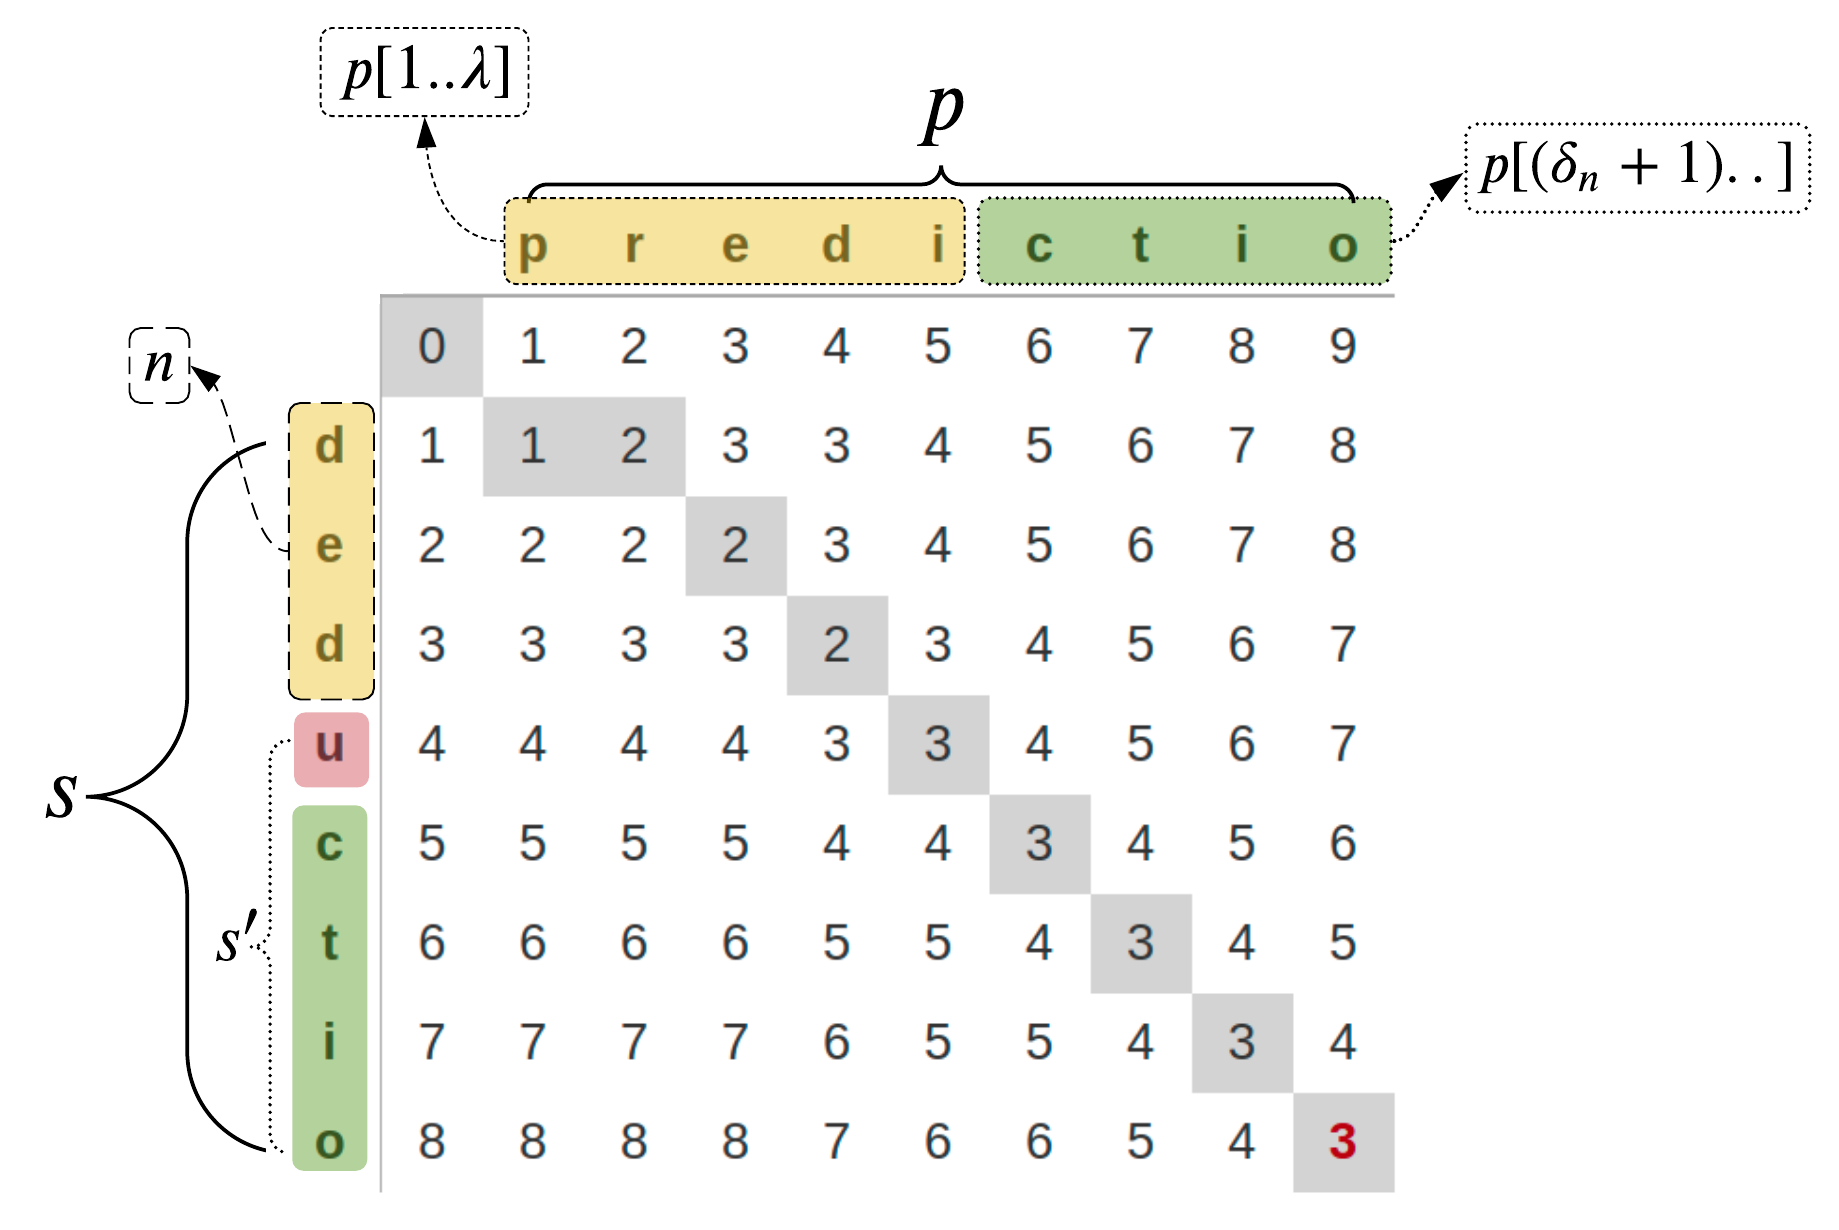
\includegraphics[width=0.94\textwidth]{figures/binary_search_counterproof.png}
    \caption{Um contra-exemplo possível que prova a imprecisão do método IP2LB, composto de uma Matriz de \textit{Levenhstein} para o cálculo de distância de edição entre $p=``predictio"$ (colunas da matriz) e a sugestão de consulta $s=``deductio"$ (linhas da matriz)}.
    \label{fig:binary_search_counterproof}
\end{figure}

A Figura~\ref{fig:binary_search_counterproof} demonstra um contra-exemplo que prova a incapacidade que o IP2LB possui de recuperar todas as sugestões de consultas similares à $p$ com até $\tau$ erros. Na figura, $\lambda = 5$, $\delta_{n}=5$, $\tau=3$. Os textos destacados em verde são, respectivamente, $p[(\delta_{n}+1)..]=``ctio"$ (o texto que é procurado pelas buscas binárias no segundo nível) e uma subcadeia $s'[2..]$ de  $s'=s[(\delta+1)..]=``uctio"$, sendo $s'[2..] = p[(\delta_{n}+1)..]$ nesse exemplo em específico. Há também os textos $``ded"$, que é o prefixo obtido a partir do caminho entre raiz da \textit{Trie} e o nó ativo de borda $n$, e $p[1..\lambda] = ``pred"$, que é o prefixo utilizado na computação de nós ativos no primeiro nível. Ambos estão coloridos em amarelo para destacar a relação entre $n$ e $p[1..\lambda]$, sendo $ed(n, p[1..\lambda] = \tau$. Além disso, há também a Matriz de \textit{Levenhstein} do cálculo de distância de edição entre $p=``predictio"$ e a sugestão de consulta $s=``deductio"$, que aliás possui o valor $3$ como podemos observar no valor da célula do canto inferior direito. Uma vez que $ed(s, p) \leq \tau$, então $s$ deve ser uma das consultas sugeridas como resposta da CATE para o prefixo de consulta $p$.

No entanto, quando o algoritmo IP2LB realiza as buscas binárias em $n$, o nó ativo de borda desse exemplo, $s$ não será incluída no conjunto de respostas para a consulta $p$ pois $p[(\delta_{n}+1)..]$, que mesmo sendo uma subcadeia de $s'$, não é encontrado nos primeiros caracteres de $s'$ como estabelecido na seção~\ref{sec:IP2LB}. Se não houvesse o caractere ``u'' (destacado em vermelho) em $s$, ou seja, se $s$ fosse $``dedctio"$, o algoritmo IP2LB consideraria $s$ como uma das sugestões válidas como resposta para a consulta. Essa falha também ocorre com outras sugestões no segundo nível do IP2LB, que por consequência não retorna alguns resultados que deveria.

Sendo assim, percebemos que não é possível aplicar a busca binária em todos os nós ativos cuja distância de edição é igual ao limiar $\tau$ sem que haja perda de resultados. Diante disso, na tentativa de resolver esse problema formulamos a hipótese de que é possível melhorar a acurácia do IP2LB restringindo a realização da busca binária para apenas alguns nós ativos de borda. Sendo $\langle n_{b}, \xi_{n_{b}}^{p[1..\lambda]}, p_{i}, \xi_{n_{b}}^{p_{i}}, \delta_{n_{b}} \rangle$ a 5-upla de um nó ativo de borda $n_b$, realizamos a busca binária nesse nó somente se $\delta_{n_{b}} = \lambda$, ou em outras palavras, se o caractere de $p[1..\lambda]$ que estava sendo processado quando $n_{b}$ foi ativado foi o $\lambda$-ésimo caractere. Essa é uma proposta de adaptação necessária para a utilização da ideia de combinar busca binária e sequencial no segundo nível, sendo uma possível resposta para a questão de pesquisa ii), apresentada na seção~\ref{sec:research-problem}. Denominamos esse método como ``IP2LRB'' (\textbf{I}C\textbf{P}AN \textbf{2}-\textit{\textbf{L}evel with \textbf{R}estricted \textbf{B}inary Search}). O algoritmo para o IP2LRB é idêntico ao Algoritmo~\ref{alg:ip2lb}, com apenas uma modificação da condição verificada na linha 6 para esta: ``$\xi_{n}^{p[1..\lambda]} = \tau \land \delta_{n} = \lambda$''.

Essa restrição faz com que a busca binária passe a ser realizada em somente $15\% \sim 40\%$ do total de nós ativos de $\Psi_{p[1..\lambda]}$, em contraste aos $75\% \sim 95\%$ do método IP2LB. O efeito disso é que o tempo de processamento de consultas do IP2LRB aproxima-se do tempo do método IP2L, porém trazendo um pouco mais de resultados que antes estavam faltando com o IP2LB. No entanto, mesmo com essa restrição o IP2LRB não consegue ter acurácia absoluta, pois ainda não traz $100\%$ dos resultados que deveria. Com isso, pensando na questão de pesquisa i) concluímos que não é possível adaptar sistemas de busca em dois níveis para tirarem proveito da busca binária no segundo nível sem que haja algum impacto na acurácia do método.